\documentclass[a4paper]{book}
\usepackage{makeidx}
\usepackage{graphicx}
\usepackage{multicol}
\usepackage{float}
\usepackage{listings}
\usepackage{color}
\usepackage{ifthen}
\usepackage[table]{xcolor}
\usepackage{textcomp}
\usepackage{alltt}
\usepackage{ifpdf}
\ifpdf
\usepackage[pdftex,
            pagebackref=true,
            colorlinks=true,
            linkcolor=blue,
            unicode
           ]{hyperref}
\else
\usepackage[ps2pdf,
            pagebackref=true,
            colorlinks=true,
            linkcolor=blue,
            unicode
           ]{hyperref}
\usepackage{pspicture}
\fi
\usepackage[utf8]{inputenc}
\usepackage{mathptmx}
\usepackage[scaled=.90]{helvet}
\usepackage{courier}
\usepackage{doxygen}
\lstset{language=C++,inputencoding=utf8,basicstyle=\footnotesize,breaklines=true,breakatwhitespace=true,tabsize=8,numbers=left }
\makeindex
\setcounter{tocdepth}{3}
\renewcommand{\footrulewidth}{0.4pt}
\begin{document}
\hypersetup{pageanchor=false}
\begin{titlepage}
\vspace*{7cm}
\begin{center}
{\Large 3D Assignment One \\[1ex]\large 1.0 }\\
\vspace*{1cm}
{\large Generated by Doxygen 1.7.3}\\
\vspace*{0.5cm}
{\small Fri Mar 4 2011 14:48:37}\\
\end{center}
\end{titlepage}
\clearemptydoublepage
\pagenumbering{roman}
\tableofcontents
\clearemptydoublepage
\pagenumbering{arabic}
\hypersetup{pageanchor=true}
\chapter{Class Index}
\doxysection{Class Hierarchy}
This inheritance list is sorted roughly, but not completely, alphabetically\+:\begin{DoxyCompactList}
\item Ogre\+::Frame\+Listener\begin{DoxyCompactList}
\item \contentsline{section}{Base\+Application}{\pageref{class_base_application}}{}
\begin{DoxyCompactList}
\item \contentsline{section}{Basic\+Tutorial\+\_\+00}{\pageref{class_basic_tutorial__00}}{}
\end{DoxyCompactList}
\end{DoxyCompactList}
\item OIS\+::Key\+Listener\begin{DoxyCompactList}
\item \contentsline{section}{Base\+Application}{\pageref{class_base_application}}{}
\end{DoxyCompactList}
\item Manual\+Object\begin{DoxyCompactList}
\item \contentsline{section}{Selection\+Rectangle}{\pageref{class_selection_rectangle}}{}
\end{DoxyCompactList}
\item OIS\+::Mouse\+Listener\begin{DoxyCompactList}
\item \contentsline{section}{Base\+Application}{\pageref{class_base_application}}{}
\end{DoxyCompactList}
\item Ogre\+Bites\+::Sdk\+Tray\+Listener\begin{DoxyCompactList}
\item \contentsline{section}{Base\+Application}{\pageref{class_base_application}}{}
\end{DoxyCompactList}
\item Ogre\+::Window\+Event\+Listener\begin{DoxyCompactList}
\item \contentsline{section}{Base\+Application}{\pageref{class_base_application}}{}
\end{DoxyCompactList}
\end{DoxyCompactList}

\chapter{Class Index}
\doxysection{Class List}
Here are the classes, structs, unions and interfaces with brief descriptions\+:\begin{DoxyCompactList}
\item\contentsline{section}{\mbox{\hyperlink{class_base_application}{Base\+Application}} }{\pageref{class_base_application}}{}
\item\contentsline{section}{\mbox{\hyperlink{class_basic_tutorial__00}{Basic\+Tutorial\+\_\+00}} \\*3D Game Programming ~\newline
My Name\+: Dai Rong Wu ~\newline
My ID\+: 310551067 ~\newline
My Email\+: \href{mailto:azusa871227@gmail.com}{\texttt{ azusa871227@gmail.\+com}} ~\newline
 Date\+: 2019/09/20 }{\pageref{class_basic_tutorial__00}}{}
\end{DoxyCompactList}

\chapter{Class Documentation}
\hypertarget{class_base_application}{
\section{BaseApplication Class Reference}
\label{class_base_application}\index{BaseApplication@{BaseApplication}}
}
Inheritance diagram for BaseApplication:\begin{figure}[H]
\begin{center}
\leavevmode
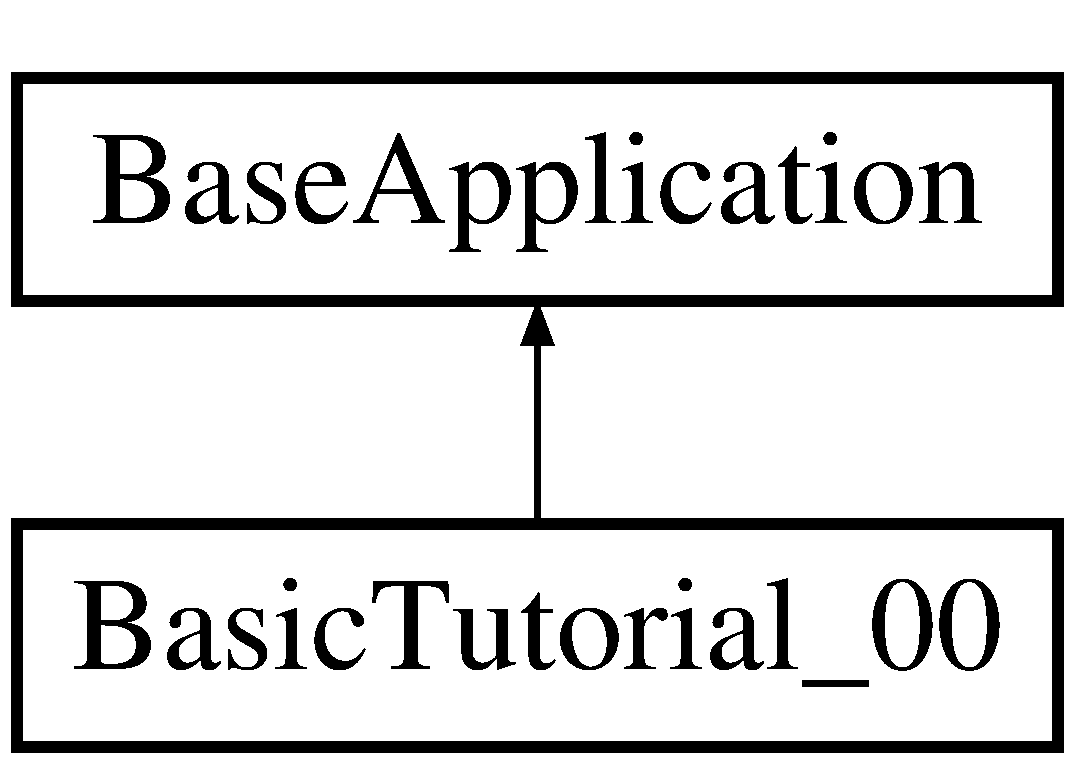
\includegraphics[height=2.000000cm]{class_base_application}
\end{center}
\end{figure}
\subsection*{Public Member Functions}
\begin{DoxyCompactItemize}
\item 
\hypertarget{class_base_application_a8a14a65a29118dd75173aa68678a05e1}{
virtual void {\bfseries go} (void)}
\label{class_base_application_a8a14a65a29118dd75173aa68678a05e1}

\end{DoxyCompactItemize}
\subsection*{Protected Member Functions}
\begin{DoxyCompactItemize}
\item 
\hypertarget{class_base_application_a5853d0e148cb85b0297a6885e1d33a89}{
virtual bool {\bfseries setup} ()}
\label{class_base_application_a5853d0e148cb85b0297a6885e1d33a89}

\item 
\hypertarget{class_base_application_a62ed46f90e9f82cc810997647a2c587e}{
virtual bool {\bfseries configure} (void)}
\label{class_base_application_a62ed46f90e9f82cc810997647a2c587e}

\item 
\hypertarget{class_base_application_ad5bc9655041e1849a4c13f444a3712bd}{
virtual void {\bfseries chooseSceneManager} (void)}
\label{class_base_application_ad5bc9655041e1849a4c13f444a3712bd}

\item 
\hypertarget{class_base_application_afa9d51527763cf9aee9cd4e1b1039d55}{
virtual void {\bfseries createCamera} (void)}
\label{class_base_application_afa9d51527763cf9aee9cd4e1b1039d55}

\item 
\hypertarget{class_base_application_aff6fd9ff1ff0978cc68f19dd65be4778}{
virtual void {\bfseries createFrameListener} (void)}
\label{class_base_application_aff6fd9ff1ff0978cc68f19dd65be4778}

\item 
\hypertarget{class_base_application_aa97beeb4059b17d0ec22eae33286ec2d}{
virtual void {\bfseries createScene} (void)=0}
\label{class_base_application_aa97beeb4059b17d0ec22eae33286ec2d}

\item 
\hypertarget{class_base_application_a365146059b25391fe400f5fdb94f011e}{
virtual void {\bfseries destroyScene} (void)}
\label{class_base_application_a365146059b25391fe400f5fdb94f011e}

\item 
\hypertarget{class_base_application_a1f8f6730cae6ec769d8730b1af48486e}{
virtual void {\bfseries createViewports} (void)}
\label{class_base_application_a1f8f6730cae6ec769d8730b1af48486e}

\item 
\hypertarget{class_base_application_ae27301702f1e5de64619a39b1929f1f9}{
virtual void {\bfseries setupResources} (void)}
\label{class_base_application_ae27301702f1e5de64619a39b1929f1f9}

\item 
\hypertarget{class_base_application_a9b77972f0f747a61e1f8ceba2ad47641}{
virtual void {\bfseries createResourceListener} (void)}
\label{class_base_application_a9b77972f0f747a61e1f8ceba2ad47641}

\item 
\hypertarget{class_base_application_aaeb764e637dd87601a81a80156659d88}{
virtual void {\bfseries loadResources} (void)}
\label{class_base_application_aaeb764e637dd87601a81a80156659d88}

\item 
\hypertarget{class_base_application_a03912a0f38b38fede7f08a2571e8fc56}{
virtual bool {\bfseries frameRenderingQueued} (const Ogre::FrameEvent \&evt)}
\label{class_base_application_a03912a0f38b38fede7f08a2571e8fc56}

\item 
\hypertarget{class_base_application_acfa977f04e435f18018ece805c1277ec}{
virtual bool {\bfseries keyPressed} (const OIS::KeyEvent \&arg)}
\label{class_base_application_acfa977f04e435f18018ece805c1277ec}

\item 
\hypertarget{class_base_application_aba5c7c9dea7a0efc58b89310bae547e5}{
virtual bool {\bfseries keyReleased} (const OIS::KeyEvent \&arg)}
\label{class_base_application_aba5c7c9dea7a0efc58b89310bae547e5}

\item 
\hypertarget{class_base_application_a126e59cb246b061e51eb6ce06a2ee8f4}{
virtual bool {\bfseries mouseMoved} (const OIS::MouseEvent \&arg)}
\label{class_base_application_a126e59cb246b061e51eb6ce06a2ee8f4}

\item 
\hypertarget{class_base_application_a9255dfc1eabefd11c474ec45a6622504}{
virtual bool {\bfseries mousePressed} (const OIS::MouseEvent \&arg, OIS::MouseButtonID id)}
\label{class_base_application_a9255dfc1eabefd11c474ec45a6622504}

\item 
\hypertarget{class_base_application_aa102c5859c14c0690c749994a446b53d}{
virtual bool {\bfseries mouseReleased} (const OIS::MouseEvent \&arg, OIS::MouseButtonID id)}
\label{class_base_application_aa102c5859c14c0690c749994a446b53d}

\item 
\hypertarget{class_base_application_afacf8a797588592ef0abbad593f10cfa}{
virtual void {\bfseries windowResized} (Ogre::RenderWindow $\ast$rw)}
\label{class_base_application_afacf8a797588592ef0abbad593f10cfa}

\item 
\hypertarget{class_base_application_ae0e37ac54a31ff6e51d58c7654ad1b90}{
virtual void {\bfseries windowClosed} (Ogre::RenderWindow $\ast$rw)}
\label{class_base_application_ae0e37ac54a31ff6e51d58c7654ad1b90}

\end{DoxyCompactItemize}
\subsection*{Protected Attributes}
\begin{DoxyCompactItemize}
\item 
\hypertarget{class_base_application_add84ba707dc6c57e6283f214b1274110}{
Ogre::Root $\ast$ {\bfseries mRoot}}
\label{class_base_application_add84ba707dc6c57e6283f214b1274110}

\item 
\hypertarget{class_base_application_a3829c6b12afe911e97e6b4524b33a38b}{
Ogre::Camera $\ast$ {\bfseries mCamera}}
\label{class_base_application_a3829c6b12afe911e97e6b4524b33a38b}

\item 
\hypertarget{class_base_application_a8a7684f4f9a57ed3089048ad1a913b2d}{
Ogre::SceneManager $\ast$ {\bfseries mSceneMgr}}
\label{class_base_application_a8a7684f4f9a57ed3089048ad1a913b2d}

\item 
\hypertarget{class_base_application_ac5d8e9c81e036897bc82f81eff8c570f}{
Ogre::RenderWindow $\ast$ {\bfseries mWindow}}
\label{class_base_application_ac5d8e9c81e036897bc82f81eff8c570f}

\item 
\hypertarget{class_base_application_a765e0df01c141a16df3178ab4f17afe6}{
Ogre::String {\bfseries mResourcesCfg}}
\label{class_base_application_a765e0df01c141a16df3178ab4f17afe6}

\item 
\hypertarget{class_base_application_a04f2fe47fa164fd78d986dc0df70b7fb}{
Ogre::String {\bfseries mPluginsCfg}}
\label{class_base_application_a04f2fe47fa164fd78d986dc0df70b7fb}

\item 
\hypertarget{class_base_application_a7faa397f4f4861ee8c361a01e90b4416}{
OgreBites::SdkTrayManager $\ast$ {\bfseries mTrayMgr}}
\label{class_base_application_a7faa397f4f4861ee8c361a01e90b4416}

\item 
\hypertarget{class_base_application_a9ae38dea6316058549151fff66a91fcd}{
OgreBites::SdkCameraMan $\ast$ {\bfseries mCameraMan}}
\label{class_base_application_a9ae38dea6316058549151fff66a91fcd}

\item 
\hypertarget{class_base_application_a6a11054ca61efdf558e0ff1b2de43a12}{
OgreBites::ParamsPanel $\ast$ {\bfseries mDetailsPanel}}
\label{class_base_application_a6a11054ca61efdf558e0ff1b2de43a12}

\item 
\hypertarget{class_base_application_ac7e861799862cb645f1d78b170aef80d}{
bool {\bfseries mCursorWasVisible}}
\label{class_base_application_ac7e861799862cb645f1d78b170aef80d}

\item 
\hypertarget{class_base_application_a755f26d3a9915aaf830750d877e39d86}{
bool {\bfseries mShutDown}}
\label{class_base_application_a755f26d3a9915aaf830750d877e39d86}

\item 
\hypertarget{class_base_application_abc9503c8462e225b5d0d55c952d9e4a9}{
OIS::InputManager $\ast$ {\bfseries mInputManager}}
\label{class_base_application_abc9503c8462e225b5d0d55c952d9e4a9}

\item 
\hypertarget{class_base_application_add9b97fbe64da2814d3af113bac58c43}{
OIS::Mouse $\ast$ {\bfseries mMouse}}
\label{class_base_application_add9b97fbe64da2814d3af113bac58c43}

\item 
\hypertarget{class_base_application_a9d6e19cf50c47379fbaae55bff28079c}{
OIS::Keyboard $\ast$ {\bfseries mKeyboard}}
\label{class_base_application_a9d6e19cf50c47379fbaae55bff28079c}

\end{DoxyCompactItemize}


The documentation for this class was generated from the following files:\begin{DoxyCompactItemize}
\item 
D:/wingo/teaching\_\-course\_\-2011/3DGameProgramming/source\_\-code/3DGame\_\-Ogre\_\-vc\_\-9\_\-v1-\/7-\/1\_\-Assigns/programs\_\-beginner/Assign\_\-01\_\-MultiViewports/source/BaseApplication.h\item 
D:/wingo/teaching\_\-course\_\-2011/3DGameProgramming/source\_\-code/3DGame\_\-Ogre\_\-vc\_\-9\_\-v1-\/7-\/1\_\-Assigns/programs\_\-beginner/Assign\_\-01\_\-MultiViewports/source/BaseApplication.cpp\end{DoxyCompactItemize}

\hypertarget{class_basic_tutorial__00}{}\doxysection{Basic\+Tutorial\+\_\+00 Class Reference}
\label{class_basic_tutorial__00}\index{BasicTutorial\_00@{BasicTutorial\_00}}


3D Game Programming ~\newline
My Name\+: Dai Rong Wu ~\newline
My ID\+: 310551067 ~\newline
My Email\+: \href{mailto:azusa871227@gmail.com}{\texttt{ azusa871227@gmail.\+com}} ~\newline
 Date\+: 2019/09/20  




{\ttfamily \#include $<$Tutorial\+Application.\+h$>$}

Inheritance diagram for Basic\+Tutorial\+\_\+00\+:\begin{figure}[H]
\begin{center}
\leavevmode
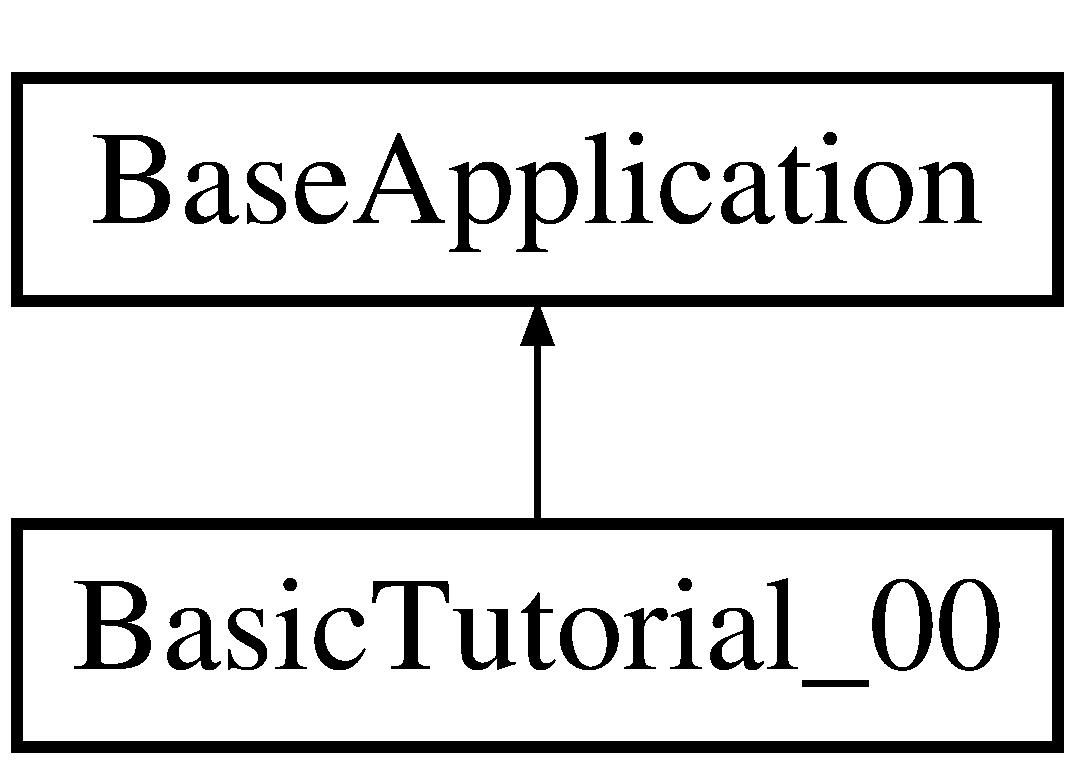
\includegraphics[height=1.909091cm]{class_basic_tutorial__00}
\end{center}
\end{figure}
\doxysubsection*{Public Member Functions}
\begin{DoxyCompactItemize}
\item 
virtual void \mbox{\hyperlink{class_basic_tutorial__00_aba97a29d983586d2dc8e108d3bccf721}{choose\+Scene\+Manager}} (void)
\item 
virtual void \mbox{\hyperlink{class_basic_tutorial__00_a1bf709417d654dffc2ea10987412b912}{create\+Camera}} (void)
\begin{DoxyCompactList}\small\item\em Call funcitons to create 2 cameras. \end{DoxyCompactList}\item 
virtual void \mbox{\hyperlink{class_basic_tutorial__00_adc2454d9f8226e0958ecf702f355846e}{create\+Viewports}} (void)
\begin{DoxyCompactList}\small\item\em call funcitons to create 2 viewports \end{DoxyCompactList}\item 
virtual void \mbox{\hyperlink{class_basic_tutorial__00_a15a3d4673724ec99077ce992f996a550}{create\+Scene}} (void)
\begin{DoxyCompactList}\small\item\em call functions to create 2 scenes \end{DoxyCompactList}\item 
\mbox{\Hypertarget{class_basic_tutorial__00_a94e281a96584a25bf57b1c5e73737c81}\label{class_basic_tutorial__00_a94e281a96584a25bf57b1c5e73737c81}} 
virtual bool {\bfseries frame\+Started} (const Ogre\+::\+Frame\+Event \&evt)
\begin{DoxyCompactList}\small\item\em Implement animation ~\newline
Implement animation when the frame refresh if the animation flag is flipped. ~\newline
. \end{DoxyCompactList}\end{DoxyCompactItemize}
\doxysubsection*{Protected Member Functions}
\begin{DoxyCompactItemize}
\item 
\mbox{\Hypertarget{class_basic_tutorial__00_a6d4684502f2f7b2cf628a975d7750d8e}\label{class_basic_tutorial__00_a6d4684502f2f7b2cf628a975d7750d8e}} 
void {\bfseries create\+Viewport\+\_\+00} (void)
\begin{DoxyCompactList}\small\item\em Create a viewport ~\newline
Create a viewport for the entire screen. ~\newline
. \end{DoxyCompactList}\item 
\mbox{\Hypertarget{class_basic_tutorial__00_a2801a2f0d91d80b471da48344d2ccccf}\label{class_basic_tutorial__00_a2801a2f0d91d80b471da48344d2ccccf}} 
void {\bfseries create\+Viewport\+\_\+01} (void)
\begin{DoxyCompactList}\small\item\em Create sub viewport ~\newline
Create Second viewport, and locate it on the left top, also set the z order. ~\newline
Also we set background color. ~\newline
. \end{DoxyCompactList}\item 
\mbox{\Hypertarget{class_basic_tutorial__00_a3479c50dbf8dc06a7ea77014eb94c6e7}\label{class_basic_tutorial__00_a3479c50dbf8dc06a7ea77014eb94c6e7}} 
void {\bfseries create\+Camera\+\_\+00} ()
\begin{DoxyCompactList}\small\item\em Create main camera ~\newline
Create main camera, set the direction, position, and clip distance, and also give it manipulation. \end{DoxyCompactList}\item 
\mbox{\Hypertarget{class_basic_tutorial__00_a8745a127adeb69fa769f832fd41412c0}\label{class_basic_tutorial__00_a8745a127adeb69fa769f832fd41412c0}} 
void {\bfseries create\+Camera\+\_\+01} ()
\begin{DoxyCompactList}\small\item\em Create sub camera ~\newline
Create the camera for second viewport, also set its direction, position, and clip distance. \end{DoxyCompactList}\item 
\mbox{\Hypertarget{class_basic_tutorial__00_aa84173e509858146cbfb98274c1ef56e}\label{class_basic_tutorial__00_aa84173e509858146cbfb98274c1ef56e}} 
void {\bfseries create\+Scene\+\_\+00} ()
\begin{DoxyCompactList}\small\item\em Create main scene ~\newline
Create main scene, including a plane, two penguins and cubes, enabling lights and shadow. ~\newline
Also set the entities\textquotesingle{}s scales, positions, and directions. ~\newline
. \end{DoxyCompactList}\item 
\mbox{\Hypertarget{class_basic_tutorial__00_aad14e1ca565797c4b7dcff31bc0e1494}\label{class_basic_tutorial__00_aad14e1ca565797c4b7dcff31bc0e1494}} 
void {\bfseries create\+Scene\+\_\+01} ()
\begin{DoxyCompactList}\small\item\em Create second scene ~\newline
Create second scene, including a plane and a cube. ~\newline
. \end{DoxyCompactList}\item 
bool \mbox{\hyperlink{class_basic_tutorial__00_adc1a0b32d78b1980b3ee51a1b1e1e69b}{key\+Pressed}} (const OIS\+::\+Key\+Event \&arg)
\begin{DoxyCompactList}\small\item\em Set key pressed events ~\newline
Set required key pressing event. ~\newline
key 1$\sim$5 for different camera position. ~\newline
key M / N for differet viewports showing on the window. ~\newline
key P for triggering animation. ~\newline
. \end{DoxyCompactList}\item 
bool \mbox{\hyperlink{class_basic_tutorial__00_aacca7a0a2a5a0e0d007b9c6c30b4941b}{key\+Released}} (const OIS\+::\+Key\+Event \&arg)
\begin{DoxyCompactList}\small\item\em Set key released events ~\newline
Didn\textquotesingle{}t modify any thing. ~\newline
. \end{DoxyCompactList}\end{DoxyCompactItemize}
\doxysubsection*{Protected Attributes}
\begin{DoxyCompactItemize}
\item 
\mbox{\Hypertarget{class_basic_tutorial__00_a6676a92b50e9b43634d4c66488537b73}\label{class_basic_tutorial__00_a6676a92b50e9b43634d4c66488537b73}} 
Ogre\+::\+Viewport $\ast$ {\bfseries m\+Viewport\+Arr} \mbox{[}8\mbox{]}
\item 
\mbox{\Hypertarget{class_basic_tutorial__00_af8d457d912286a98c0975c52d4faf910}\label{class_basic_tutorial__00_af8d457d912286a98c0975c52d4faf910}} 
Ogre\+::\+Camera $\ast$ {\bfseries m\+Camera\+Arr} \mbox{[}8\mbox{]}
\item 
\mbox{\Hypertarget{class_basic_tutorial__00_a603779b6087698c57b7989e16d8a9b93}\label{class_basic_tutorial__00_a603779b6087698c57b7989e16d8a9b93}} 
Ogre\+::\+Scene\+Manager $\ast$ {\bfseries m\+Scene\+Mgr\+Arr} \mbox{[}8\mbox{]}
\item 
\mbox{\Hypertarget{class_basic_tutorial__00_a700c07f924c71e9fa1885a46f599d934}\label{class_basic_tutorial__00_a700c07f924c71e9fa1885a46f599d934}} 
Ogre\+Bites\+::\+Sdk\+Camera\+Man $\ast$ {\bfseries m\+Camera\+Man\+Arr} \mbox{[}8\mbox{]}
\end{DoxyCompactItemize}


\doxysubsection{Detailed Description}
3D Game Programming ~\newline
My Name\+: Dai Rong Wu ~\newline
My ID\+: 310551067 ~\newline
My Email\+: \href{mailto:azusa871227@gmail.com}{\texttt{ azusa871227@gmail.\+com}} ~\newline
 Date\+: 2019/09/20 

This is an assignment of 3D Game Programming I didn\textquotesingle{}t modify any thing in this headfile. This class define the function we use and the members. 

\doxysubsection{Member Function Documentation}
\mbox{\Hypertarget{class_basic_tutorial__00_aba97a29d983586d2dc8e108d3bccf721}\label{class_basic_tutorial__00_aba97a29d983586d2dc8e108d3bccf721}} 
\index{BasicTutorial\_00@{BasicTutorial\_00}!chooseSceneManager@{chooseSceneManager}}
\index{chooseSceneManager@{chooseSceneManager}!BasicTutorial\_00@{BasicTutorial\_00}}
\doxysubsubsection{\texorpdfstring{chooseSceneManager()}{chooseSceneManager()}}
{\footnotesize\ttfamily void Basic\+Tutorial\+\_\+00\+::choose\+Scene\+Manager (\begin{DoxyParamCaption}\item[{void}]{ }\end{DoxyParamCaption})\hspace{0.3cm}{\ttfamily [virtual]}}



Reimplemented from \mbox{\hyperlink{class_base_application}{Base\+Application}}.

\mbox{\Hypertarget{class_basic_tutorial__00_a1bf709417d654dffc2ea10987412b912}\label{class_basic_tutorial__00_a1bf709417d654dffc2ea10987412b912}} 
\index{BasicTutorial\_00@{BasicTutorial\_00}!createCamera@{createCamera}}
\index{createCamera@{createCamera}!BasicTutorial\_00@{BasicTutorial\_00}}
\doxysubsubsection{\texorpdfstring{createCamera()}{createCamera()}}
{\footnotesize\ttfamily void Basic\+Tutorial\+\_\+00\+::create\+Camera (\begin{DoxyParamCaption}\item[{void}]{ }\end{DoxyParamCaption})\hspace{0.3cm}{\ttfamily [virtual]}}



Call funcitons to create 2 cameras. 



Reimplemented from \mbox{\hyperlink{class_base_application}{Base\+Application}}.

\mbox{\Hypertarget{class_basic_tutorial__00_a15a3d4673724ec99077ce992f996a550}\label{class_basic_tutorial__00_a15a3d4673724ec99077ce992f996a550}} 
\index{BasicTutorial\_00@{BasicTutorial\_00}!createScene@{createScene}}
\index{createScene@{createScene}!BasicTutorial\_00@{BasicTutorial\_00}}
\doxysubsubsection{\texorpdfstring{createScene()}{createScene()}}
{\footnotesize\ttfamily void Basic\+Tutorial\+\_\+00\+::create\+Scene (\begin{DoxyParamCaption}\item[{void}]{ }\end{DoxyParamCaption})\hspace{0.3cm}{\ttfamily [virtual]}}



call functions to create 2 scenes 



Implements \mbox{\hyperlink{class_base_application}{Base\+Application}}.

\mbox{\Hypertarget{class_basic_tutorial__00_adc2454d9f8226e0958ecf702f355846e}\label{class_basic_tutorial__00_adc2454d9f8226e0958ecf702f355846e}} 
\index{BasicTutorial\_00@{BasicTutorial\_00}!createViewports@{createViewports}}
\index{createViewports@{createViewports}!BasicTutorial\_00@{BasicTutorial\_00}}
\doxysubsubsection{\texorpdfstring{createViewports()}{createViewports()}}
{\footnotesize\ttfamily void Basic\+Tutorial\+\_\+00\+::create\+Viewports (\begin{DoxyParamCaption}\item[{void}]{ }\end{DoxyParamCaption})\hspace{0.3cm}{\ttfamily [virtual]}}



call funcitons to create 2 viewports 



Reimplemented from \mbox{\hyperlink{class_base_application}{Base\+Application}}.

\mbox{\Hypertarget{class_basic_tutorial__00_adc1a0b32d78b1980b3ee51a1b1e1e69b}\label{class_basic_tutorial__00_adc1a0b32d78b1980b3ee51a1b1e1e69b}} 
\index{BasicTutorial\_00@{BasicTutorial\_00}!keyPressed@{keyPressed}}
\index{keyPressed@{keyPressed}!BasicTutorial\_00@{BasicTutorial\_00}}
\doxysubsubsection{\texorpdfstring{keyPressed()}{keyPressed()}}
{\footnotesize\ttfamily bool Basic\+Tutorial\+\_\+00\+::key\+Pressed (\begin{DoxyParamCaption}\item[{const OIS\+::\+Key\+Event \&}]{arg }\end{DoxyParamCaption})\hspace{0.3cm}{\ttfamily [protected]}, {\ttfamily [virtual]}}



Set key pressed events ~\newline
Set required key pressing event. ~\newline
key 1$\sim$5 for different camera position. ~\newline
key M / N for differet viewports showing on the window. ~\newline
key P for triggering animation. ~\newline
. 



Reimplemented from \mbox{\hyperlink{class_base_application}{Base\+Application}}.

\mbox{\Hypertarget{class_basic_tutorial__00_aacca7a0a2a5a0e0d007b9c6c30b4941b}\label{class_basic_tutorial__00_aacca7a0a2a5a0e0d007b9c6c30b4941b}} 
\index{BasicTutorial\_00@{BasicTutorial\_00}!keyReleased@{keyReleased}}
\index{keyReleased@{keyReleased}!BasicTutorial\_00@{BasicTutorial\_00}}
\doxysubsubsection{\texorpdfstring{keyReleased()}{keyReleased()}}
{\footnotesize\ttfamily bool Basic\+Tutorial\+\_\+00\+::key\+Released (\begin{DoxyParamCaption}\item[{const OIS\+::\+Key\+Event \&}]{arg }\end{DoxyParamCaption})\hspace{0.3cm}{\ttfamily [protected]}, {\ttfamily [virtual]}}



Set key released events ~\newline
Didn\textquotesingle{}t modify any thing. ~\newline
. 



Reimplemented from \mbox{\hyperlink{class_base_application}{Base\+Application}}.



The documentation for this class was generated from the following files\+:\begin{DoxyCompactItemize}
\item 
D\+:/hw01\+\_\+310551067/programs/3\+DGP\+\_\+201909\+\_\+01\+\_\+\+Multi\+Viewports\+\_\+\+Template/source/Tutorial\+Application.\+h\item 
D\+:/hw01\+\_\+310551067/programs/3\+DGP\+\_\+201909\+\_\+01\+\_\+\+Multi\+Viewports\+\_\+\+Template/source/Tutorial\+Application.\+cpp\end{DoxyCompactItemize}

\printindex
\end{document}
